\documentclass[10pt,a4paper]{article}

\usepackage[utf8]{inputenc}
\usepackage[T1]{fontenc}
\usepackage[brazil]{babel}
\usepackage[margin=1.85cm, top=2.1cm, bottom=2.0cm]{geometry}
\usepackage{graphicx}
\usepackage{booktabs}
\usepackage{tabularx}
\usepackage{array}
\usepackage{amsmath}
\usepackage{xcolor}
\usepackage{colortbl}
\usepackage{fancyhdr}
\usepackage{lastpage}
\usepackage{titlesec}
\usepackage{enumitem}
\usepackage{tikz}
\usetikzlibrary{arrows.meta, positioning, shapes.geometric}
\usepackage[most]{tcolorbox}
\usepackage{hyperref}
\usepackage{caption}

% ==============================================================================
% PALETA INSTITUCIONAL & ESTILO EXECUTIVO
% ==============================================================================
\definecolor{uelgreen}{RGB}{15, 80, 35}
\definecolor{ueldark}{RGB}{10, 52, 22}
\definecolor{ueltint}{RGB}{241, 247, 243}
\definecolor{slate}{RGB}{45, 55, 72}
\definecolor{muted}{RGB}{100, 110, 120}
\definecolor{bordergray}{RGB}{210, 218, 222}

\hypersetup{
    colorlinks=true,
    linkcolor=uelgreen,
    urlcolor=uelgreen,
    pdftitle={Relatório Técnico — Mineração de Dados (2COP024)},
    pdfauthor={Lucas Silva, Marcos Beregula}
}

% Títulos de seção elegantes com barra inferior
\titleformat{\section}
  {\large\bfseries\color{uelgreen}}
  {\thesection.}{0.5em}{}
  [\vspace{-0.4em}{\color{uelgreen}\rule{\textwidth}{0.8pt}}]

\titleformat{\subsection}
  {\normalsize\bfseries\color{slate}}
  {\thesubsection}{0.5em}{}

\titlespacing*{\section}{0pt}{10pt}{5pt}
\titlespacing*{\subsection}{0pt}{7pt}{3pt}

% Cabeçalho e rodapé
\pagestyle{fancy}
\fancyhf{}
\renewcommand{\headrulewidth}{0.5pt}
\renewcommand{\headrule}{\hbox to\headwidth{\color{uelgreen}\leaders\hrule height \headrulewidth\hfill}}
\renewcommand{\footrulewidth}{0.4pt}
\renewcommand{\footrule}{\hbox to\headwidth{\color{bordergray}\leaders\hrule height \footrulewidth\hfill}}
\fancyhead[L]{\footnotesize\color{slate}\textbf{Mineração de Dados (2COP024)} \textbar\ Previsão de Avaliações Negativas}
\fancyhead[R]{\footnotesize\color{muted}UEL --- 30/11/2026}
\fancyfoot[L]{\footnotesize\color{muted}Lucas Silva e Marcos Beregula}
\fancyfoot[R]{\footnotesize\color{muted}Página \thepage\ de \pageref{LastPage}}

% Listas compactas
\setlist[itemize]{leftmargin=1.3em, itemsep=1.5pt, topsep=2pt, parsep=0pt}
\setlist[enumerate]{leftmargin=1.5em, itemsep=1.5pt, topsep=2pt, parsep=0pt}

% Captions
\captionsetup{font={footnotesize,color=slate}, labelfont={bf,color=uelgreen}, skip=4pt}

% Caixas executivas
\newtcolorbox{execbox}[1]{
    colback=ueltint,
    colframe=uelgreen,
    boxrule=0.8pt,
    arc=2pt,
    left=8pt, right=8pt, top=5pt, bottom=5pt,
    fonttitle=\small\bfseries\color{white},
    coltitle=white,
    colbacktitle=uelgreen,
    title=#1
}

\newtcolorbox{kpibox}[2]{
    enhanced,
    colback=white,
    colframe=uelgreen!55,
    boxrule=0.7pt,
    arc=2pt,
    left=3pt, right=3pt, top=7pt, bottom=4pt,
    halign=center,
    valign=center,
    width=#1,
    nobeforeafter,
    title=\centering\scriptsize\bfseries#2,
    colbacktitle=ueltint,
    coltitle=uelgreen,
    attach boxed title to top center={yshift=-2.2mm},
    boxed title style={boxrule=0.5pt, colframe=uelgreen!55, arc=1.5pt, left=4pt, right=4pt, top=1pt, bottom=1pt}
}

\newcolumntype{P}[1]{>{\raggedright\arraybackslash}p{#1}}

\begin{document}
\thispagestyle{empty}

% ==============================================================================
% CABEÇALHO EXECUTIVO (PÁGINA 1)
% ==============================================================================
\noindent
\begin{minipage}[c]{0.73\textwidth}
    \raggedright
    {\normalsize\bfseries\color{uelgreen} UNIVERSIDADE ESTADUAL DE LONDRINA (UEL)}\\[2pt]
    {\small\bfseries\color{slate} Disciplina: Mineração de Dados (2COP024)}\\[6pt]
    {\Large\bfseries\color{ueldark} Previsão de Avaliações Negativas em E-commerce de Livros}\\[2pt]
    {\normalsize\bfseries\color{uelgreen} Mineração de Texto com TF-IDF e Linear SVM}
\end{minipage}
\hfill
\begin{minipage}[c]{0.23\textwidth}
    \raggedleft
    
\includegraphics[width=\textwidth]{contexto/Logo UEL.png}
\end{minipage}

\vspace{5pt}
{\color{uelgreen}\rule{\textwidth}{1.5pt}}
\vspace{3pt}

\noindent
{\small\color{slate}\textbf{Autores:} Lucas Silva e Marcos Beregula \hfill \textbf{Data:} 30 de novembro de 2026}\\[2pt]
{\footnotesize\color{muted}\textbf{Entregável:} Relatório Técnico Executivo (4 a 6 páginas) --- Projeto Integrador}

\vspace{8pt}

% Faixa de KPIs Executivos
\noindent
\begin{kpibox}{0.238\textwidth}{Recall (Classe Negativa)}
    {\Large\bfseries\color{uelgreen} 77,70\%}\\
    {\scriptsize\color{muted} 230 de 296 críticas reais}
\end{kpibox}\hfill
\begin{kpibox}{0.238\textwidth}{F1-Score (Teste Cego)}
    {\Large\bfseries\color{uelgreen} 0,7044}\\
    {\scriptsize\color{muted} Precisão: 64,43\%}
\end{kpibox}\hfill
\begin{kpibox}{0.238\textwidth}{PR-AUC (Desbalanceado)}
    {\Large\bfseries\color{uelgreen} 0,7843}\\
    {\scriptsize\color{muted} 9,7$\times$ acima do aleatório}
\end{kpibox}\hfill
\begin{kpibox}{0.238\textwidth}{ROC-AUC Global}
    {\Large\bfseries\color{uelgreen} 0,9689}\\
    {\scriptsize\color{muted} Alta separabilidade}
\end{kpibox}

\vspace{6pt}

% ==============================================================================
% 1. PERGUNTA DE PESQUISA E CONTEXTO DE NEGÓCIO
% ==============================================================================
\section{Pergunta de Pesquisa e Contexto de Negócio}

Em grandes plataformas de comércio eletrônico, o volume diário de avaliações publicadas pelos consumidores inviabiliza a leitura e a triagem manual de cada comentário. Nesse ambiente, o custo operacional dos erros de classificação é fortemente \textbf{assimétrico}: deixar de identificar um cliente insatisfeito (\textit{Falso Negativo}) resulta em cancelamentos silenciosos (\textit{churn}), perda de retenção e degradação da reputação do catálogo.

\begin{execbox}{Pergunta Central de Pesquisa}
\small \textit{``É possível prever se uma avaliação de livro da Amazon será negativa com base exclusivamente no texto da resenha, utilizando técnicas clássicas de mineração de texto em cenário severamente desbalanceado?''}
\end{execbox}

Para responder de forma empiricamente rigorosa, o problema foi formulado como \textbf{classificação binária supervisionada sobre texto livre} (concatenação de título e corpo da resenha), adotando protocolo estrito contra vazamento de dados (\textit{data leakage}) e métricas orientadas à classe minoritária de interesse (\textbf{F1-Score}, \textbf{Recall} e \textbf{PR-AUC}).

% ==============================================================================
% 2. BASE DE DADOS E ENGENHARIA DO ALVO
% ==============================================================================
\section{Base de Dados e Engenharia da Variável-Alvo}

Utilizou-se a coleção oficial \textbf{Amazon Reviews 2023 (categoria \textit{Books})}, mantida pelo McAuley Lab (UCSD). Para garantir reprodutibilidade e eficiência de memória, extraíram-se $20.000$ avaliações via \textit{streaming} HTTP direto com algoritmo de \textbf{amostragem por reservatório limitado} (\textit{Bounded Reservoir Sampling}, semente \texttt{20261109}).

A variável-alvo binária \texttt{is\_negative} foi construída por polarização explícita das notas originais (1 a 5 estrelas), visando separar manifestações claras de satisfação e insatisfação:
\begin{itemize}
    \item \textbf{Classe 1 (Negativa --- notas 1,0 e 2,0):} $1.478$ resenhas (\textbf{8,04\%} da base elegível).
    \item \textbf{Classe 0 (Positiva --- notas 4,0 e 5,0):} $16.910$ resenhas (\textbf{91,96\%} da base elegível).
    \item \textbf{Exclusão da nota 3,0:} $1.612$ avaliações neutras removidas por reunirem simultaneamente elogios e críticas, evitando fronteiras semânticas ambíguas.
\end{itemize}

A base elegível final totalizou \textbf{18.388 avaliações}, caracterizando um desbalanceamento aproximado de \textbf{11,4 avaliações positivas para cada negativa} (Figura~\ref{fig:eda}). Em função dessa proporção, o uso da acurácia simples como critério principal foi descartado, pois um classificador trivial obteria $\approx 92\%$ de acurácia sem detectar nenhuma crítica real.

\begin{figure}[htbp]
    \centering
    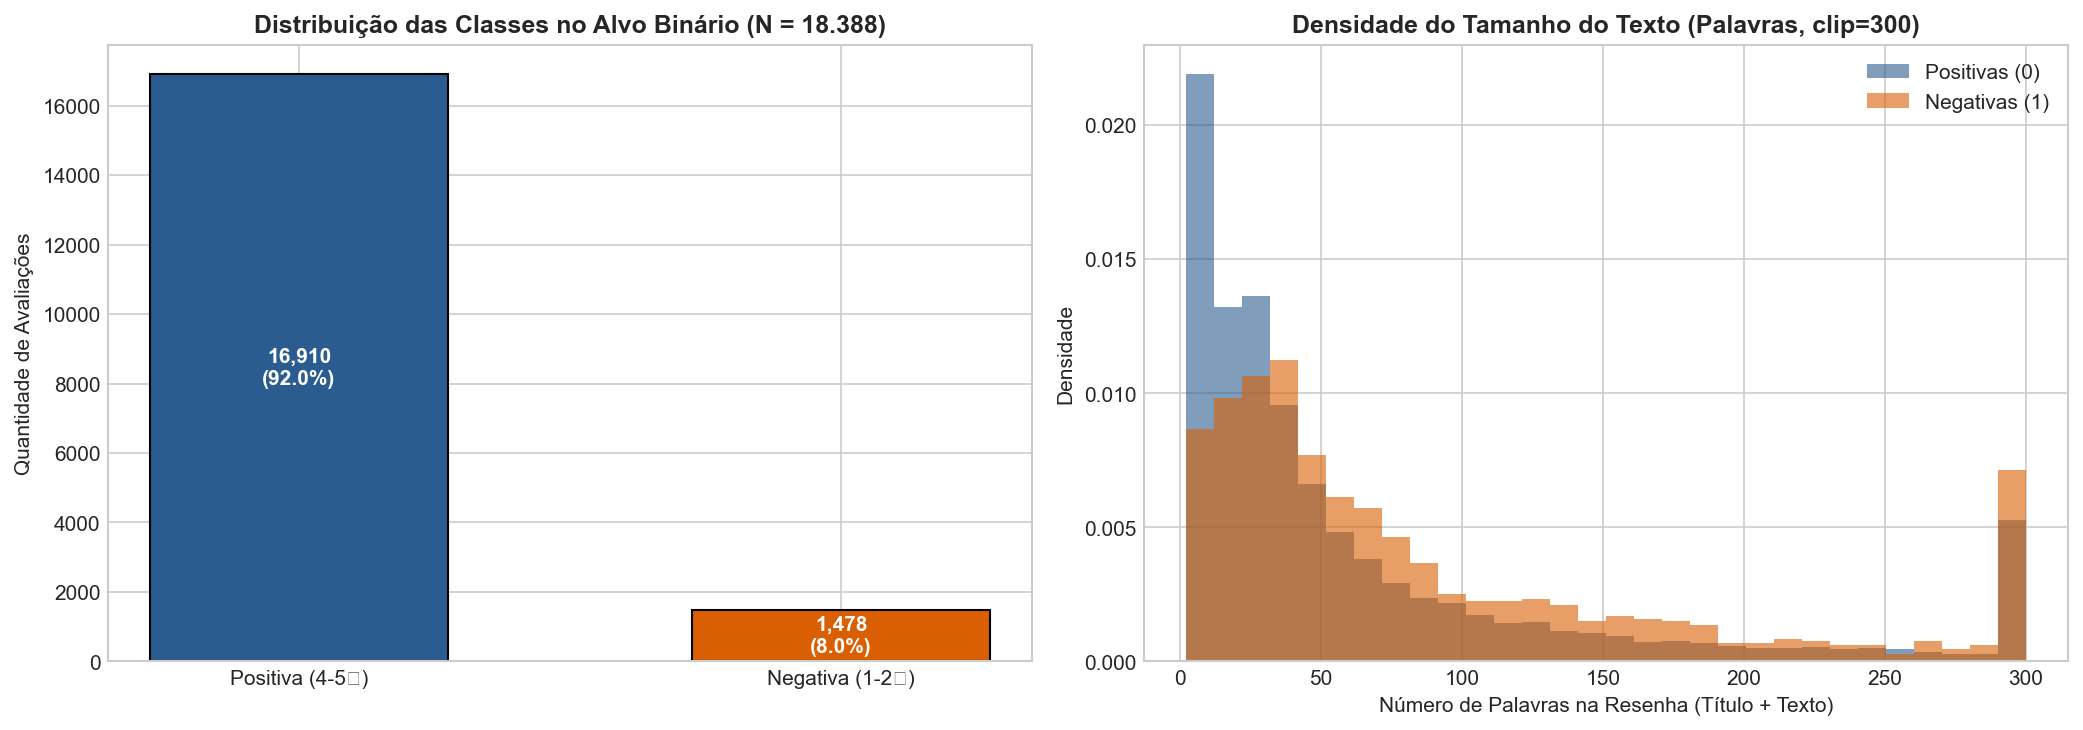
\includegraphics[width=0.84\textwidth]{outputs/figura1_distribuicao_classes_eda.png}
    \caption{Distribuição das classes após binarização ($N = 18.388$) e densidade do número de palavras por resenha.}
    \label{fig:eda}
\end{figure}

% ==============================================================================
% 3. O QUE FOI FEITO: PIPELINE ANTI-VAZAMENTO E MODELAGEM
% ==============================================================================
\section{O que foi Feito: Pipeline, Representação Textual e Modelagem}

Todo o experimento foi encapsulado em objetos \texttt{Pipeline} do \texttt{scikit-learn} para impedir qualquer vazamento de estatísticas do conjunto de teste para o treino (Figura~\ref{fig:pipeline}).

\begin{figure}[htbp]
\centering
\begin{tikzpicture}[
    node distance=0.45cm,
    etapa/.style={rectangle, draw=uelgreen, thick, rounded corners=2pt, minimum width=2.25cm, minimum height=0.85cm, align=center, font=\scriptsize, fill=ueltint},
    seta/.style={->, thick, uelgreen}
]
\node[etapa] (s1) {\textbf{1. Split 80/20}\\Estratificado (\texttt{seed=42})};
\node[etapa, right=of s1] (s2) {\textbf{2. TF-IDF}\\(\texttt{fit} só no Treino)};
\node[etapa, right=of s2] (s3) {\textbf{3. Seleção/Redução}\\Filter, L1, SVD};
\node[etapa, right=of s3] (s4) {\textbf{4. Classificador}\\SVM / LogReg};
\node[etapa, right=of s4] (s5) {\textbf{5. Teste Cego}\\$N = 3.678$ intocado};
\draw[seta] (s1) -- (s2);
\draw[seta] (s2) -- (s3);
\draw[seta] (s3) -- (s4);
\draw[seta] (s4) -- (s5);
\end{tikzpicture}
\caption{Fluxo experimental ponta a ponta com isolamento estrito do conjunto de teste ($20\%$).}
\label{fig:pipeline}
\end{figure}

\begin{itemize}
    \item \textbf{Partição Congelada (80/20):} $14.710$ avaliações para treino/validação cruzada e $3.678$ mantidas congeladas para avaliação única final.
    \item \textbf{Engenharia de Texto e TF-IDF:} concatenação \texttt{review\_full = title + [espaço] + text}, capturando a síntese emocional dos títulos. O vetorizador \texttt{TfidfVectorizer} utilizou unigramas e bigramas (\texttt{ngram\_range=(1, 2)}) para preservar negações (ex.: \textit{``not good''}, \textit{``waste time''}), filtros \texttt{min\_df=3} e \texttt{max\_df=0.90}, escala sublinear ($1 + \log(\text{TF})$) e limite de $5.000$ atributos.
    \item \textbf{Classificadores Supervisionados:} comparação em validação cruzada estratificada de 5 dobras (5-Fold CV) entre \textbf{Linear SVM} (\texttt{LinearSVC}, margem máxima / \textit{Hinge Loss}, $C = 0{,}5$) e \textbf{Regressão Logística} (\textit{Log-Loss}), ambos com \texttt{class\_weight='balanced'}.
    \item \textbf{Seleção vs. Redução Dimensional:} comparação controlada sobre o classificador campeão entre o \textit{Baseline} completo ($5.000$ termos), seleção \textit{Filter} (\texttt{SelectKBest} $\chi^2$, $1.500$ termos), seleção \textit{Embedded} (\texttt{SelectFromModel} com penalização Lasso L1) e redução densa (\texttt{TruncatedSVD} / PCA com $100$ componentes).
\end{itemize}

% ==============================================================================
% 4. RESULTADOS OBTIDOS
% ==============================================================================
\section{Resultados Obtidos}

\subsection{Comparação de Modelos e Seleção vs. Redução de Atributos (5-Fold CV)}

Na validação cruzada sobre os $14.710$ exemplos de treino, o \textbf{Linear SVM} obteve F1-Score médio de \textbf{0,6874} ($\sigma = \pm 0{,}0189$), superando ligeiramente a \textbf{Regressão Logística} (\textbf{0,6851}, $\sigma = \pm 0{,}0142$) e confirmando sua adequação clássica a matrizes esparsas de alta dimensão.

A Tabela~\ref{tab:selecao} e a Figura~\ref{fig:selecao} demonstram o impacto das estratégias de dimensionalidade sobre o Linear SVM. Os métodos de \textbf{seleção discreta} (\textit{Embedded} L1 e \textit{Filter} $\chi^2$) preservaram mais de $94\%$ do desempenho original mesmo descartando até $70\%$ do vocabulário. Em contraste, a \textbf{redução densa via TruncatedSVD} derrubou o F1-Score em quase $30\%$ ($0{,}4862$), pois a projeção em combinações lineares ortogonais dilui termos raros e altamente discriminativos (como \textit{``waste''} e \textit{``horrible''}) no ruído de fundo do vocabulário comum.

\begin{table}[htbp]
\centering
\footnotesize
\caption{Desempenho em 5-Fold CV (Linear SVM) comparando seleção e redução de atributos.}
\label{tab:selecao}
\begin{tabularx}{\textwidth}{P{2.0cm} P{3.9cm} c c X}
\toprule
\rowcolor{ueltint} \textbf{Versão} & \textbf{Técnica Aplicada} & \textbf{F1-Score (CV)} & \textbf{Retenção} & \textbf{Diagnóstico Técnico} \\
\midrule
\textbf{Baseline} & Sem seleção ($5.000$ $n$-gramas) & \textbf{0,6874} & \textbf{100,0\%} & Preserva a cauda longa lexical \\
\textbf{Embedded} & \texttt{SelectFromModel} (Lasso L1) & 0,6614 & 96,2\% & Elimina termos redundantes \\
\textbf{Filter} & \texttt{SelectKBest} ($\chi^2$, $1.500$ termos) & 0,6472 & 94,2\% & Alta compactação com perda leve \\
\textbf{Redução (PCA)} & \texttt{TruncatedSVD} ($100$ comp.) & \textbf{0,4862} & 70,7\% & Degradação severa do sinal esparso \\
\bottomrule
\end{tabularx}
\end{table}

\begin{figure}[htbp]
    \centering
    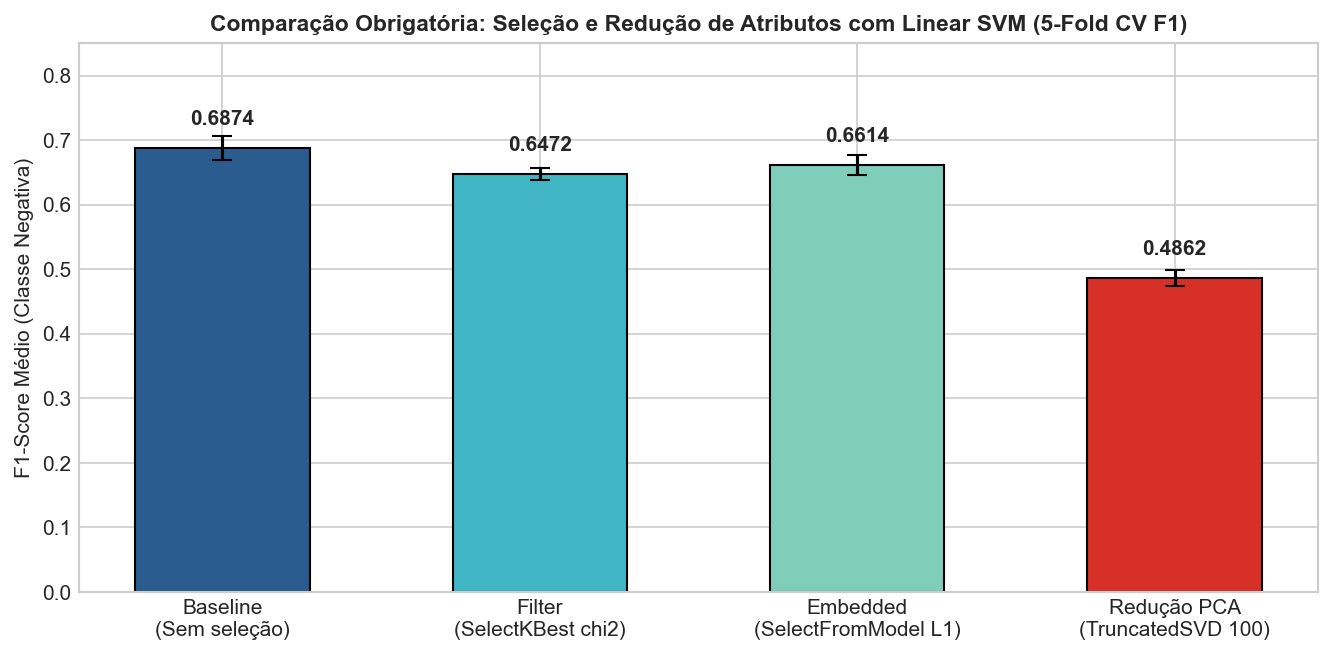
\includegraphics[width=0.78\textwidth]{outputs/figura3_comparacao_selecao_reducao.png}
    \caption{Comparação do F1-Score (5-Fold CV) entre preservação lexical, seleção de atributos e redução via SVD.}
    \label{fig:selecao}
\end{figure}

\subsection{Avaliação Final no Conjunto de Teste Cego ($N = 3.678$)}

Aplicado o modelo campeão (\texttt{TfidfVectorizer} + \texttt{LinearSVC} balanceado) uma única vez ao conjunto de teste congelado, obtiveram-se os resultados da Tabela~\ref{tab:teste} e da Figura~\ref{fig:teste}. O modelo capturou \textbf{230 Verdadeiros Positivos} de insatisfação contra apenas \textbf{66 Falsos Negativos}, alcançando \textbf{Recall de 77,70\%} e \textbf{PR-AUC de 0,7843} (quase dez vezes superior ao baseline aleatório de $0{,}0805$).

\begin{table}[htbp]
\centering
\footnotesize
\caption{Métricas oficiais do classificador campeão no conjunto de teste independente ($N = 3.678$).}
\label{tab:teste}
\begin{tabularx}{\textwidth}{P{4.2cm} c X}
\toprule
\rowcolor{ueltint} \textbf{Métrica} & \textbf{Valor} & \textbf{Interpretação Operacional} \\
\midrule
\textbf{Recall (Classe Negativa)} & \textbf{77,70\%} & Detecta quase $8$ em cada $10$ resenhas insatisfeitas reais \\
\textbf{Precisão (Classe Negativa)} & \textbf{64,43\%} & Cerca de $2$ em cada $3$ alertas gerados são críticos reais \\
\textbf{F1-Score (Classe Negativa)} & \textbf{0,7044} & Equilíbrio robusto sob desbalanceamento de $8{,}04\%$ \\
\textbf{PR-AUC (Precision-Recall)} & \textbf{0,7843} & Ganho de $\approx 9{,}7\times$ sobre o baseline aleatório ($0{,}0805$) \\
\textbf{ROC-AUC} & \textbf{0,9689} & Excelente separabilidade ordinal entre avaliações \\
\bottomrule
\end{tabularx}
\end{table}

\begin{figure}[htbp]
    \centering
    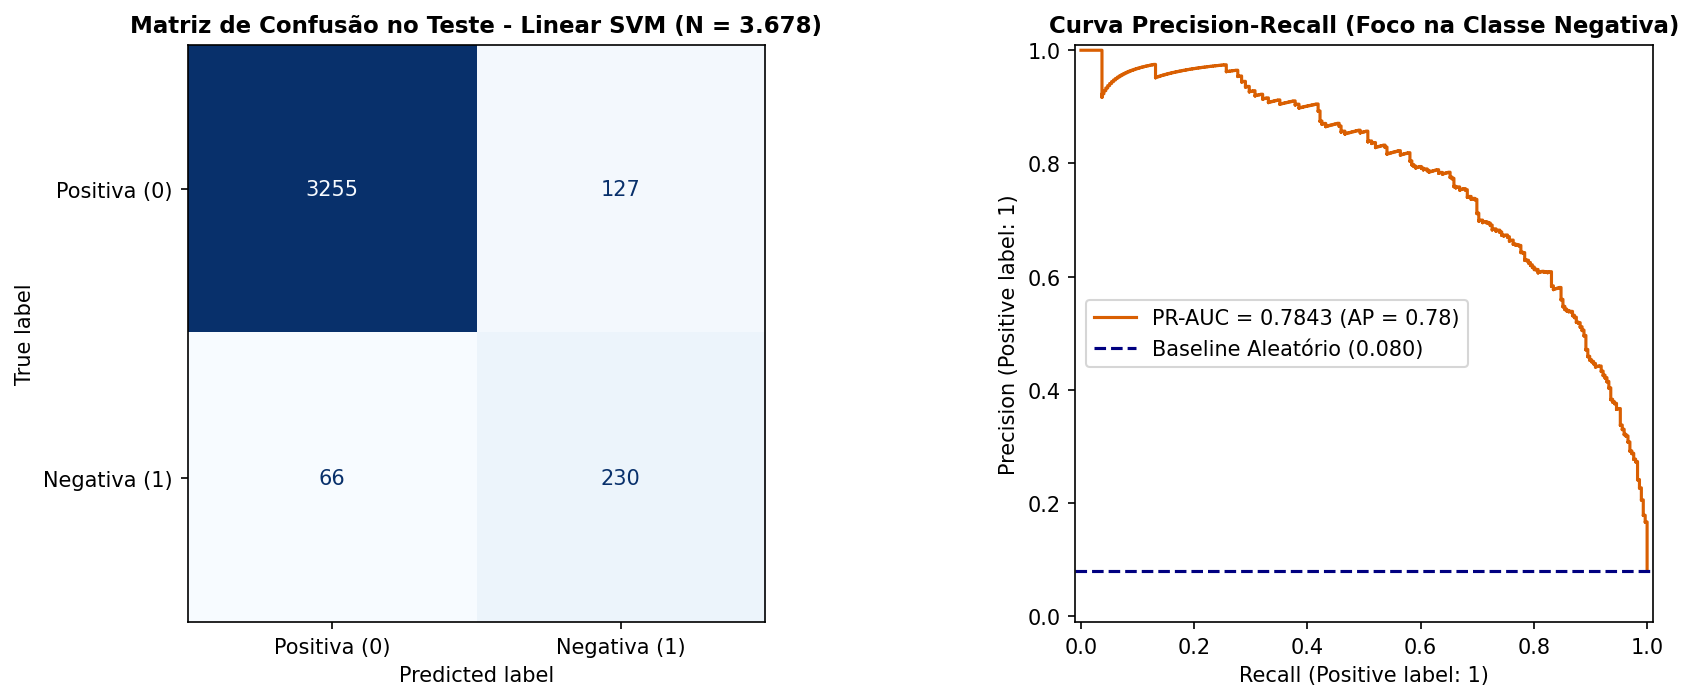
\includegraphics[width=0.90\textwidth]{outputs/figura4_avaliacao_matriz_confusao_pr_roc.png}
    \caption{Matriz de confusão, curva Precision-Recall e curva ROC obtidas no conjunto de teste cego.}
    \label{fig:teste}
\end{figure}

\subsection{Diagnóstico de Ruído nos Rótulos (VADER) e Interpretabilidade}

Como auditoria complementar, aplicou-se o léxico de sentimento VADER ($|\text{score}| \ge 0{,}60$) para sinalizar potenciais contradições entre a nota atribuída e o texto escrito (Figura~\ref{fig:vader_coef}, esquerda). Foram sinalizados \textbf{887 casos suspeitos (4,82\%)} (ex.: nota $1\star$ com texto aparentemente elogioso), tratados estritamente como \textbf{suspeitas diagnósticas} e não como erros comprovados. Em um estudo de ablação removendo essas ocorrências apenas do treino (mantendo o teste intacto), o F1-Score variou de \textbf{0,7044} (treino normal, $14.710$ ex.) para \textbf{0,6988} (treino filtrado, $13.999$ ex.), demonstrando que o Linear SVM já possui estabilidade natural ao ruído de rotulagem.

A inspeção dos pesos do hiperplano do SVM (Figura~\ref{fig:vader_coef}, direita) confirma a coerência semântica do modelo: os principais termos que impulsionam a classe negativa são \textit{``waste''}, \textit{``not''}, \textit{``poor''}, \textit{``disappointed''}, \textit{``boring''}, \textit{``return''}, \textit{``waste time''}, \textit{``worst''}, \textit{``terrible''} e \textit{``awful''}; para a classe positiva destacam-se \textit{``great''}, \textit{``excellent''}, \textit{``loved''}, \textit{``must read''}, \textit{``best''}, \textit{``highly recommend''} e \textit{``wonderful''}.

\begin{figure}[htbp]
    \centering
    \begin{minipage}[c]{0.48\textwidth}
        \centering
        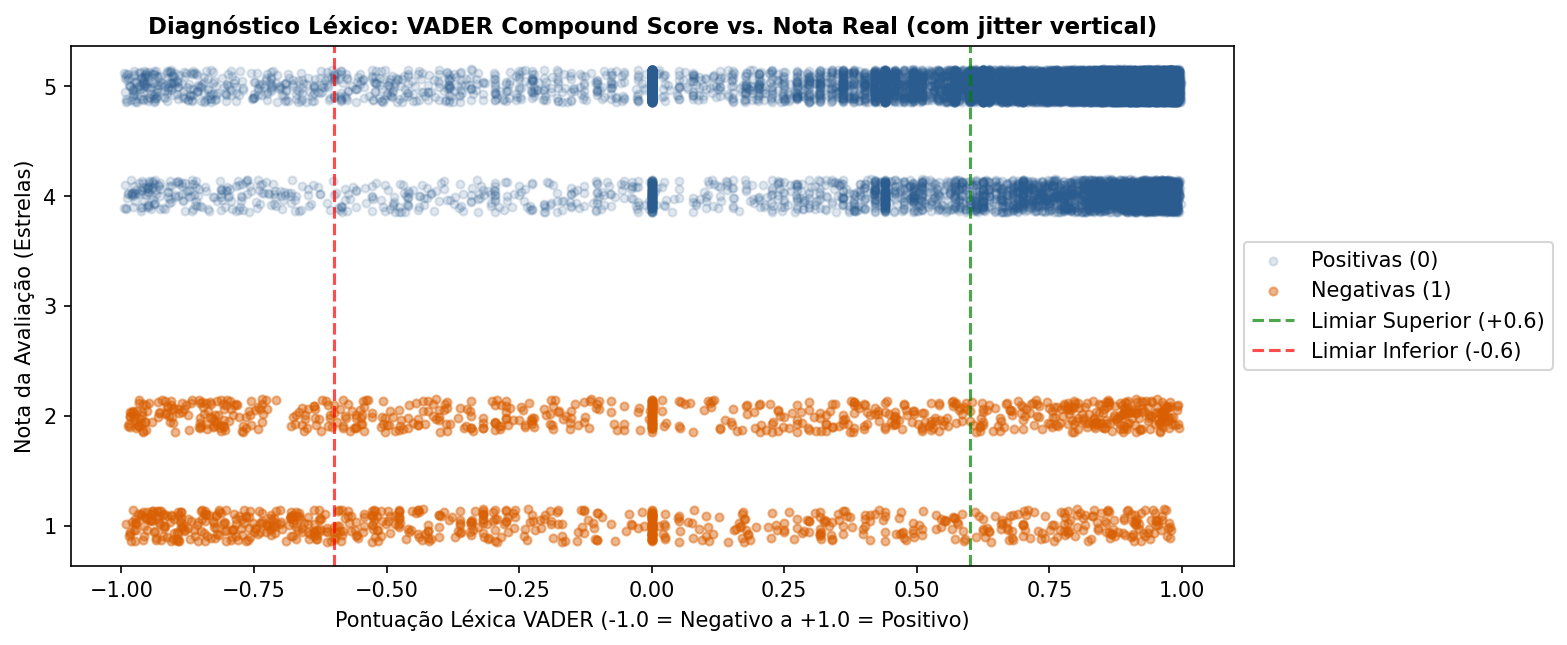
\includegraphics[width=\textwidth]{outputs/figura2_diagnostico_divergencias_vader.png}
    \end{minipage}\hfill
    \begin{minipage}[c]{0.49\textwidth}
        \centering
        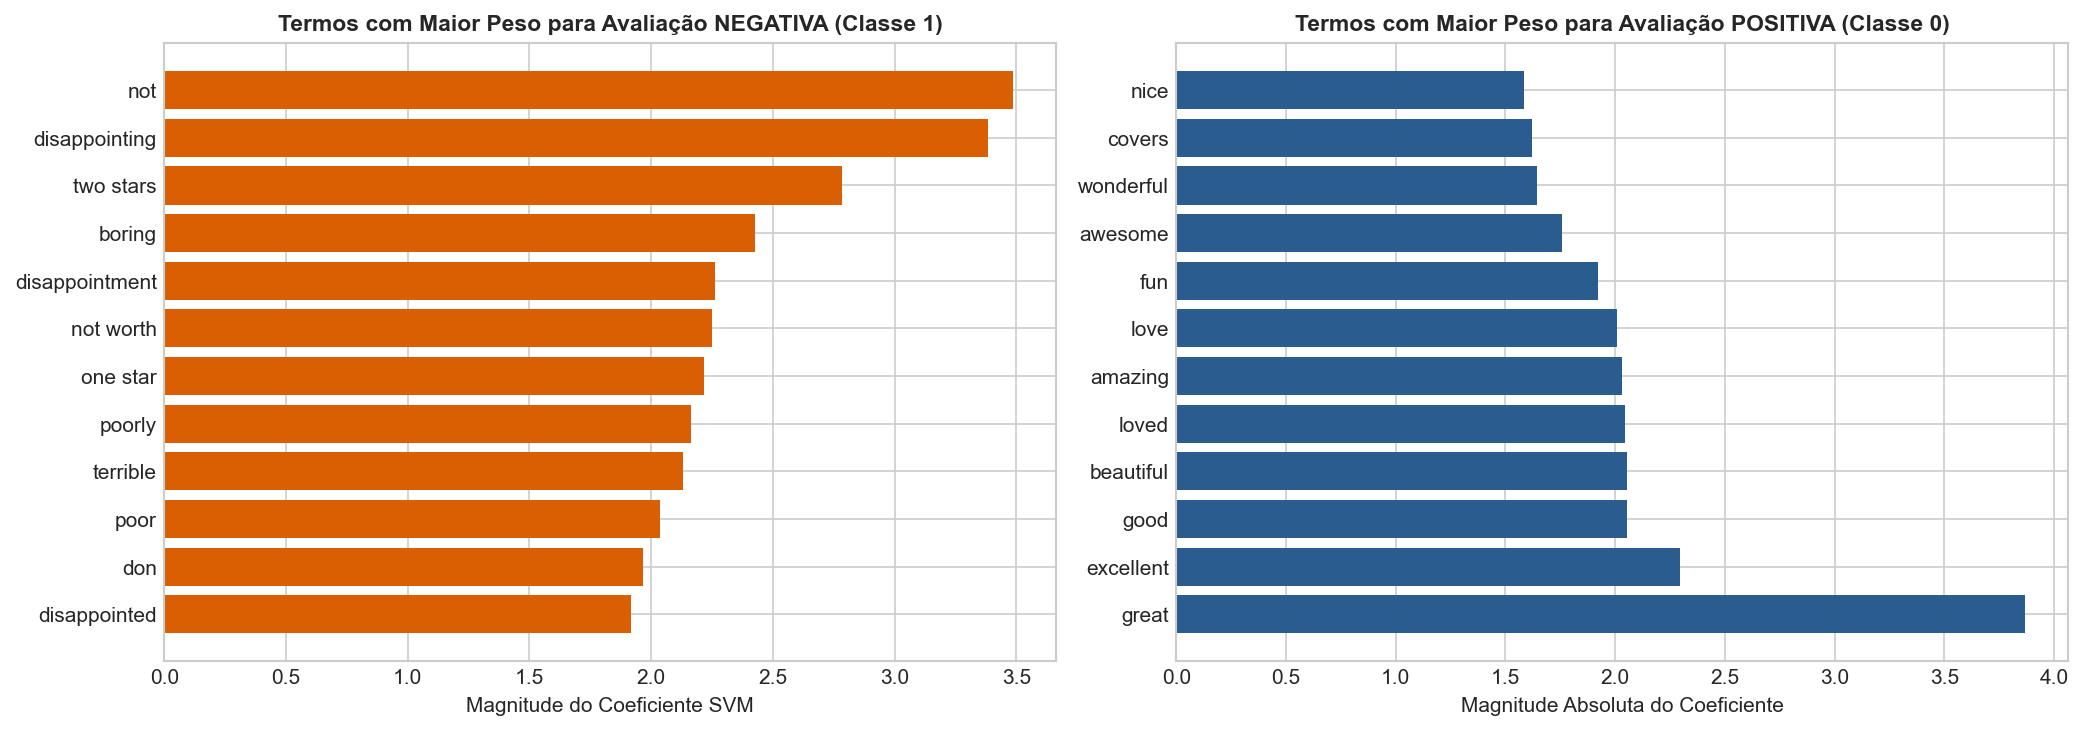
\includegraphics[width=\textwidth]{outputs/figura5_coeficientes_palavras_chave.png}
    \end{minipage}
    \caption{À esquerda: diagnóstico de divergências léxicas via VADER. À direita: principais coeficientes do hiperplano SVM.}
    \label{fig:vader_coef}
\end{figure}

% ==============================================================================
% 5. LIMITES E CUIDADOS METODOLÓGICOS
% ==============================================================================
\section{Limites do Estudo}

\begin{itemize}
    \item \textbf{Exclusão da classe neutra (nota 3,0):} a remoção de $1.612$ resenhas intermediárias torna o classificador altamente eficaz para extremos de polaridade, mas não modela textos mistos sem retreinamento específico.
    \item \textbf{Ausência de calibração probabilística nativa:} o \texttt{LinearSVC} produz escores de margem (\texttt{decision\_function}), exigindo calibração posterior (ex.: \texttt{CalibratedClassifierCV}) caso o sistema operacional necessite de probabilidades calibradas.
    \item \textbf{Limitações de modelos puramente lexicais (\textit{Bag-of-$n$-grams}):} embora bigramas capturem negações simples, ironias extensas, sarcasmo contextual e dependências semânticas de longa distância fogem ao escopo do TF-IDF linear.
    \item \textbf{Domínio restrito e viés de amostra:} os pesos aprendidos refletem o vocabulário específico de livros da Amazon em língua inglesa, exigindo reajuste antes de transferência para outras categorias ou idiomas.
\end{itemize}

% ==============================================================================
% 6. CONCLUSÃO
% ==============================================================================
\section{Conclusão}

\begin{execbox}{Resposta Conclusiva}
\small \textbf{Sim.} Os experimentos comprovam que é tecnicamente viável prever avaliações negativas de livros exclusivamente a partir do texto da resenha, atingindo \textbf{77,70\% de Recall}, \textbf{0,7044 de F1-Score} e \textbf{0,7843 de PR-AUC} no teste cego sob desbalanceamento severo ($8{,}04\%$).
\end{execbox}

\vspace{4pt}
Como principais contribuições técnicas do trabalho destacam-se: (i) a construção de um fluxo inteiramente livre de vazamento de dados; (ii) a comprovação empírica de que a \textbf{preservação e seleção lexical superam drasticamente a redução dimensional densa (SVD)} em textos esparsos; e (iii) a demonstração via ablação de que o Linear SVM balanceado é naturalmente resiliente ao ruído ocasional de rótulos. Como próximos passos para implantação em produção, recomenda-se a calibração de probabilidades e o ajuste fino do limiar de decisão em função do custo marginal de atendimento no SAC.

\vspace{6pt}
\noindent{\scriptsize\color{muted}\textbf{Repositório e Reprodutibilidade:} Código-fonte, notebooks e metadados disponíveis em \url{https://github.com/luticaa/mineracao-de-dados-projeto-final}. Base: \textit{Amazon Reviews 2023} (Hou et al., McAuley Lab / UCSD); \textit{VADER} (Hutto \& Gilbert, ICWSM 2014); \textit{Scikit-learn} (Pedregosa et al., JMLR 2011).}

\end{document}
